\chapter{Particles reconstruction and simulation}
~~~~The final state of a coherent (incoherent) DVCS event consists of three 
particles: an electron, a $^4$He (a proton), and a real photon. To identify the 
DVCS events, we first identify, individually, the different particles of 
interest. Then, events with three detected final-state particles will be 
further filtered by imposing the energy-momentum conservation laws, as will be 
presented in the following chapter.\\ 


Even after imposing the conservation laws, the DVCS sample will not have 
100$\%$ truly DVCS events. In our kinematical region, the main contamination to 
our DVCS channels comes from the electroproduction of neutral pions. For 
instance, in the coherent $\pi^0$-electroproduction, when one of the two-photon 
decay of the $\pi^{0}$ passes the DVCS requirements, it will be counted as a 
DVCS event. Thus, these events have to be subtracted before looking to any DVCS 
observable. For this purpose, we perform a technique in which we combine the 
measured exclusive $\pi^0$-electroproduction data sample with a Monte-Carlo 
simulation to evaluate the background in the selected DVCS sample. For this 
technique, we need to identify the experimental $\pi^0$s that come in the 
coherent and the incoherent $\pi^0$-electroproduction channels.\\
 
 
In this chapter, we presents the procedures carried out to identify the 
final-state particles of interest, the Monte-Carlo simulation we used, and the 
kinematic corrections we applied on the particles.

\section{Particles identification}
     
\subsection{Electron identification} \label{Electron_identification}
~~~~The electron detection triggers the data acquisition system to record data 
from all the sub-detectors of CLAS. In this analysis, a particle which passes 
the following set of criteria is assumed to be a good electron.
  
\paragraph{Initial requirements}

\begin{itemize}
\item Negative charge: the torus magnet generates a field which has mainly azimuthal components. Hence, the trajectory of a negative particle will be bent towards the beam line direction without changing azimuth. Consequently, information on its charge is accessible from the curvature of its trajectory.           

\item $(DC_{stat}, EC_{stat}, SC_{stat}, CC_{stat}) > 0$: these status variables are linked to the number of hits and the thresholds in the different sub-detectors of CLAS. Thus, we select the electrons which have positive status in the different sub-detectors as a first step to reduce the noise in the data sample.

\item $stat$ > 0: this variable is positive if the trajectory of a particle passes the two steps of the tracking in the DCs, Hit-Based Tracking (HBT) and Time-Based Tracking (TBT).

\item Momentum cut ($p_{e^{-}}$ > 0.8 GeV/c): during the data acquisition, the 
   EC threshold was set to 200 $mV$ corresponding to electrons having a minimum 
   momentum of about 0.7 GeV/c. In this analysis, we apply a conservative cut 
   of 0.8 GeV/c to be above this threshold.

\item Vertex cut: the target is centered at -64 cm with respect to the center of CLAS. Figure \ref{fig:z_cut} shows the reconstructed z-vertices for the collected negative particles. One sees two sharp peaks corresponding to the two aluminum windows at the ends of the target. These particles have to be rejected as they originate from outside the target. As will be emphasized later, we need an accurate determination of the electron's vertex to ensure the correspondence between the final-state particles, which all have to originate from the same point.       
 
\begin{figure}[tp]
\centering
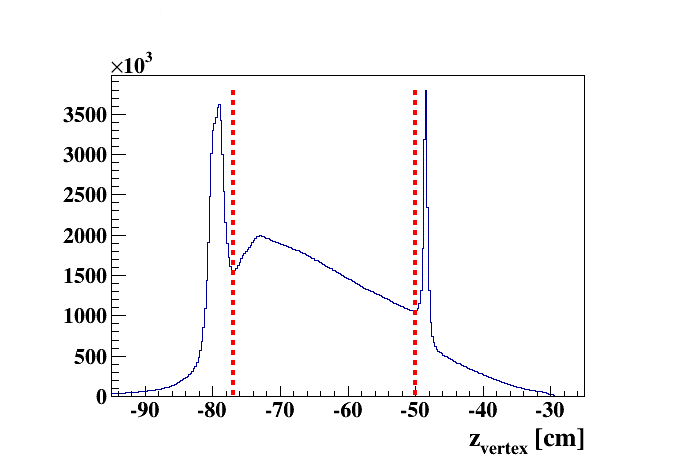
\includegraphics[scale=0.43]{fig_analysis/Z_e.png}
\caption{The reconstructed longitudinal vertex of the collected negative particles. The two dashed red lines represent the chosen cut, -77 cm < $z_{vertex}$ < -50 cm, to eliminate the particles which originate from the windows and outside the target.} 
\label{fig:z_cut}
\end{figure}

\paragraph{Fiducial cuts}
~\\
~\\
~~~~Some regions of CLAS have to be excluded from the analysis to ensure an accurate detection of the different particles. For instance, an electron that hits the edge of the EC will have only part of its electromagnetic shower contained within the detector. Also, the structure of the torus magnet divides CLAS into six separate sectors, which makes edge effects non-negligible. For this reason, the following set of fiducial cuts is applied:      
 
\begin{itemize}
\item EC fiducial cut: each EC has a triangular shape with its three sides labelled as U,V and W. We apply a set of cuts (60 cm < $U$, $V$ < 360 cm, $W$ < 390 cm) to reject the electrons which hit the EC close to the edges, as shown in figure \ref{fig:EC_cut}.
\begin{figure}[tbp]
\hspace{-0.2in}
%\includegraphics[scale=0.22]{fig_analysis/EC.png}
%\includegraphics[scale=0.28]{fig_analysis/el_u.png}
%\includegraphics[scale=0.28]{fig_analysis/el_v.png}
%\includegraphics[scale=0.28]{fig_analysis/el_w.png}
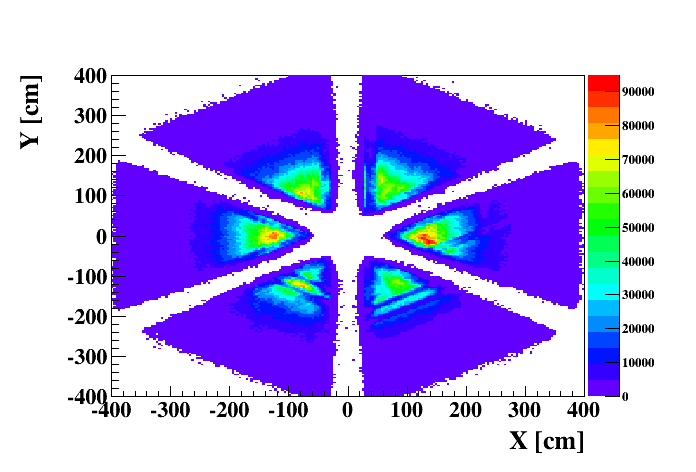
\includegraphics[scale=0.35]{fig_analysis/EC_XY_el_1.png}
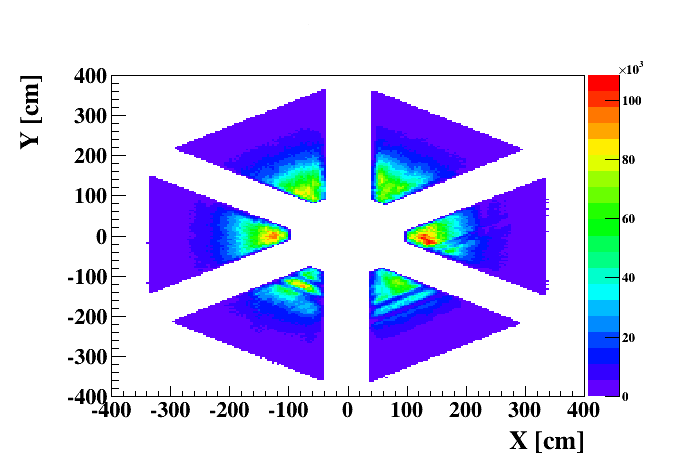
\includegraphics[scale=0.35]{fig_analysis/EC_XY_el_2.png}
\caption{On the left: XY distribution for the negative particles in the EC before the $U$, $V$ and $W$ cuts. On the right: the same distribution is plotted after the cuts. $X$ and $Y$ are the coordinates in the EC with respect to the center of CLAS.} 
\label{fig:EC_cut}
\end{figure}

\begin{figure}[tbp]
\hspace{-0.2in}
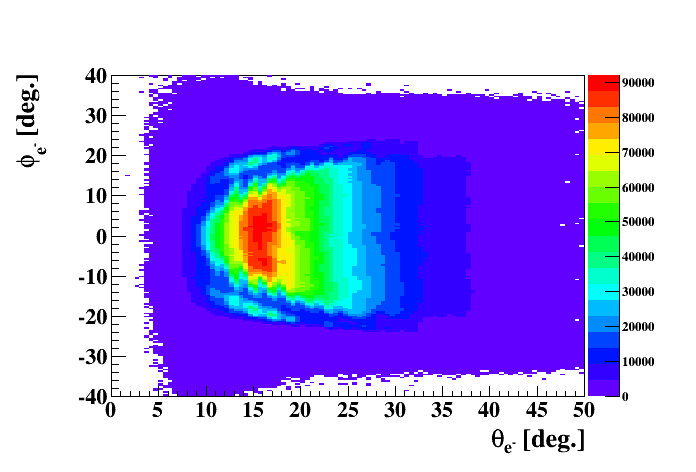
\includegraphics[scale=0.35]{fig_analysis/CC_el_phi_theta_1.png}
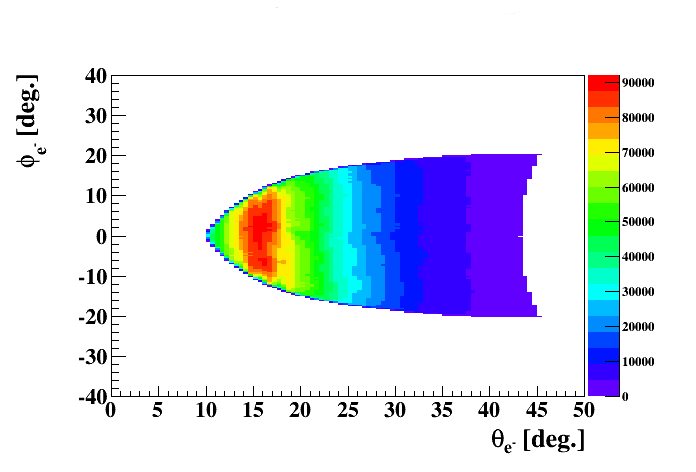
\includegraphics[scale=0.35]{fig_analysis/CC_el_phi_theta_2.png}
\caption{Azimuthal angle as a function of polar angle for the negative particles before (left) and after (right) applying the CC fiducial cut. The angles are calculated with respect to the center of each sector in CLAS.} 
\label{fig:CC_cut}
\end{figure}

\item CC fiducial cut: in reference \cite{CCref}, G. Adams {\it et al.} have studied the efficiency of the CCs. They found that within the fiducial regions, which are defined by the edges of the CCs mirrors, the detection efficiency is stable and is around 98$\%$. Outside the fiducial regions, the efficiency shows strong variations. In reference \cite{Osipenko}, M. Osipenko {\it et al.} have developed a coordinate system to represent the CC hits with respect to the center of each sector in CLAS. In this frame, the CCs mirror edges can be defined as:\\
\begin{multline}  
\phi_{e}  = -63.32792 +11.05609\cdot \theta_{e} -0.6344957\cdot \theta^{2}_{e} +1.873895*10^{-2}\cdot \theta^{3}_{e} \\
- 2.762131*10^{-2}\cdot \theta^{4}_{e}+1.604035*10^{-2}\cdot \theta^{5}_{e}. ~~~~~~~~~~~~~~~~~~~~~~~~~
\end{multline}
Based on these works, we reject all the hits located outside the mirror edges. Figure \ref{fig:CC_cut} shows an illustration of this cut.



\item IC shadow cut: this cut originates from the location of the IC in front of the innermost part of the DCs. The electrons which are produced at polar angles lower than 14$^\circ$ will hit the IC. The left plot of figure \ref{fig:IC_cut} illustrates this effect, and the right plot shows the effect of the cut we apply.
\begin{figure}[tbp]
\hspace{-0.2in}
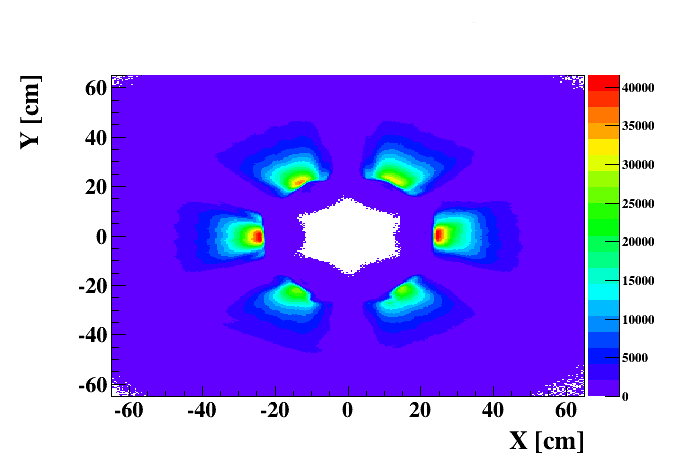
\includegraphics[scale=0.35]{fig_analysis/el_DC_IC_XY_1.png}
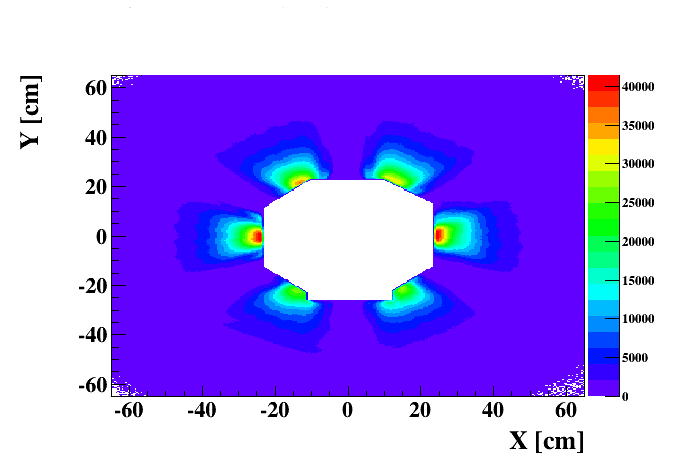
\includegraphics[scale=0.35]{fig_analysis/el_DC_IC_XY_2.png}
\caption{On the left: XY distribution for all the negative particles in the first region of the DC before applying the IC shadow cut. On the right: the same distribution after the cut.} 
\label{fig:IC_cut}
\end{figure}


\item DC fiducial cut: the DCs have low detection efficiency at the edges because only part of the tracks are detected \cite{DCref}. So we apply a fiducial cut to reject the particles at the edges. The left plot of figure \ref{fig:IC_cut} shows the XY distribution of all the negative particles in DC1. The result of applying the DC fiducial cut can be seen in figure \ref{fig:DC_cut}.  
\begin{figure}[tbp]
\centering
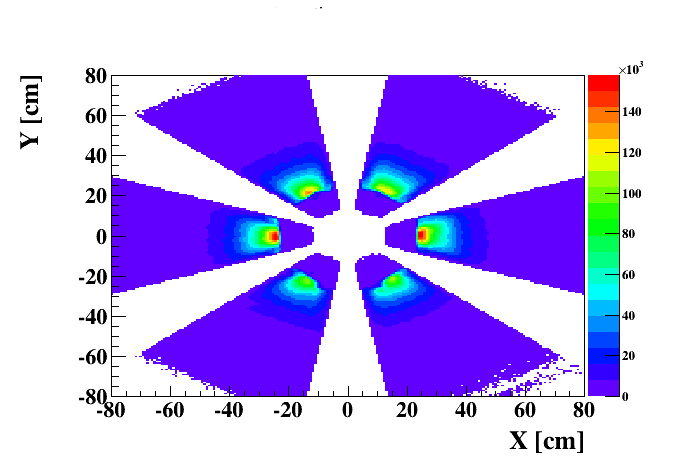
\includegraphics[scale=0.35]{fig_analysis/DC_el_2.png}
\caption{ XY distribution for all the negative particles in DC1 after applying the DC fiducial cut.} 
\label{fig:DC_cut}
\end{figure}

\end{itemize}

\paragraph{EC energy cuts}
~\\
~\\
~~~~The Minimum Ionizing particles (MIPs), such as pions, deposit constant 
amounts of energy per distance while traversing the EC.  In contrast, the 
showering particles, such as electrons and photons, deposit energies 
proportional to their momenta. We use two energy cuts to clean the electrons 
from the main contamination, i.e.  $\pi^{-}$s.
\begin{itemize}
\item Minimum deposited energy:
   the inner and the outer parts of the EC have thicknesses 15 cm and 24 cm, 
   respectively. The simulations show that pions deposit a constant energy 
   amount of 2 MeV/cm, independently of their momenta. Figure 
   \ref{fig:Einner_cut} shows the deposited energy in the outer part of the EC 
   (EC$_{out}$) as a function of the energy deposited in the inner part 
   (EC$_{in}$), after the fiducial cuts. On the x-axis, one can see a clear 
   region, around 30 MeV, that comes mainly from the negative pions, which 
   deposit 2 MeV/cm along the 15 cm thickness of the inner EC. We use a cut of 
   60 MeV on EC$_{in}$ to reject these particles. 
   
\item An additional cut, correlating the measured deposited energy and the momentum, is applied. Figure \ref{fig:etot_p_cut} shows the ratio of the total deposited energy in the ECs (EC$_{tot}$ = EC$_{in}$ + EC$_{out}$) to the momentum ($p$) as a function of $p$. One notices that EC$_{tot}$/p varies slightly with the momentum due to variations in the efficiencies of the DC and EC. We apply 2.5$\sigma$ cuts around the mean ($\mu$) to select the good electrons, using to the following parametrizations of the mean ($\mu$) and the width ($\sigma$):
\begin{eqnarray}
\mu (p) = 0.256084 +0.0432374\cdot p -0.00914180\cdot p^{2} +0.00081589 \cdot p^{3} \\
\sigma (p) = 0.0572976 -0.0272689\cdot p +0.008576\cdot p^{2} -0.00097998\cdot p^{3}
\end{eqnarray}

   
\begin{figure}[tp]
\begin{minipage}[c]{.46\linewidth}
\hspace{-0.3in}
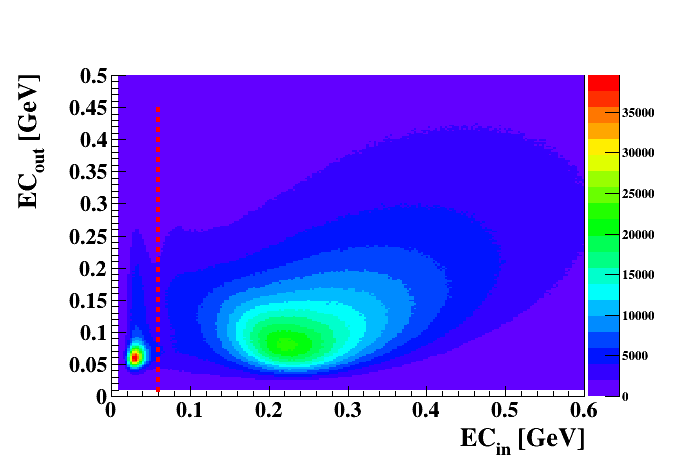
\includegraphics[height=6.2cm]{fig_analysis/eco_eci.png}
\caption{Deposited energies in the EC: $E_{out}$ as a function of $E_{in}$. The dashed red line represents a 60 MeV cut on EC$_{in}$ to reject the $\pi^{-}$s. } 
\label{fig:Einner_cut}
\end{minipage} \hfill
\begin{minipage}[c]{.46\linewidth}
\hspace{-0.2in}
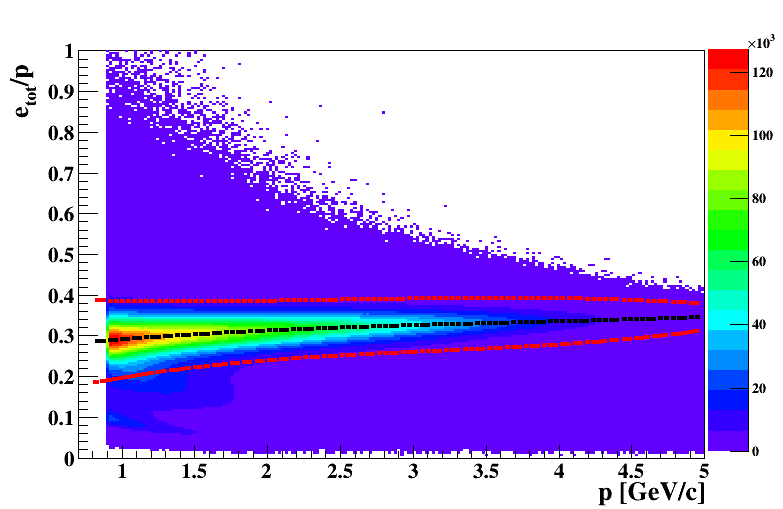
\includegraphics[height=5.3cm]{fig_analysis/etot_p.png}
\caption{$E_{tot}/p$ as a function of $p$. The black dashed line represents the mean value of $E_{tot}/p$ as a function of $p$. The red dashed lines represent the $2.5 \sigma$ cuts. } 
\label{fig:etot_p_cut}
\end{minipage}
\end{figure}

\end{itemize}

\paragraph{CC cut}
~\\
~\\
~~~~The Cherenkov counters have been designed to separate electrons from pions below 2.5 GeV/c momentum. In this region, the pions are not supposed to produce photoelectrons. However, low momentum $\delta$-electrons can be produced from the diffusion of the pions in the Cherenkov gas. These $\delta$-electrons produce a small number of photoelectrons. Figure \ref{fig:Nphe_cut} shows the distributions of the number of photoelectrons ($nphe$) produced by the negative particles for three different stages of the electron selection. \\

   
One sees from figure \ref{fig:Nphe_cut} that the single-photoelectron peak is 
strongly reduced after applying the energy cuts. We conclude that the particles 
causing the single-photoelectrons peak are linked to particles with low 
deposited energy in the EC$_{in}$, figure \ref{fig:Einner_cut}. We apply a 
final cut on the red distribution in figure \ref{fig:Nphe_cut} ($nphe$~>~2), 
and we assume that the negative particles which pass all the previous 
requirements and produce more than 2 photoelectrons in the CC are good 
electrons.
\begin{figure}[tpb]
\centering
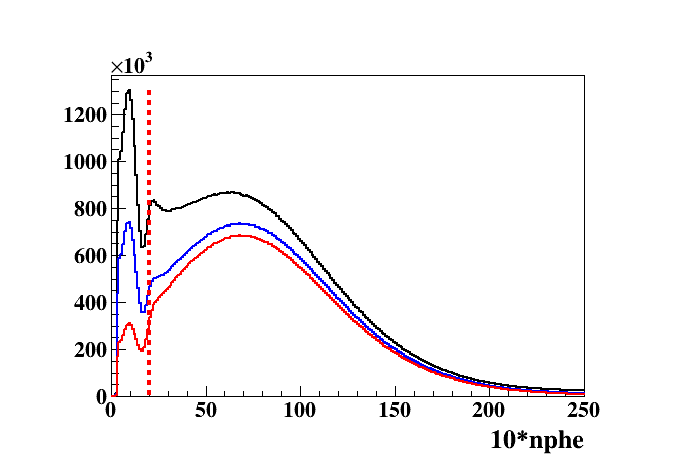
\includegraphics[height=7.0cm]{fig_analysis/nphe_all.png}
\caption{Distribution of number of photoelectrons emitted by negative particles 
in the CC ($nphe\cdot$10). The black curve represents the distribution after 
the initial cuts, the blue curve is after the geometrical cuts and the red 
curve is after applying all the cuts including the EC energy cuts. The dashed 
red line represents the cut we apply ($nphe$~>~2) to select the good 
electrons.} \label{fig:Nphe_cut}
\end{figure}

%\begin{figure}[tbp]
%\centering
%\includegraphics[height=6.8cm]{fig_analysis/e_phi_theta_4.png}
%\caption{$\phi$ vs. $\theta$ distribution of the selected electrons.}
%\label{fig:e_phi_theta_4}
%\end{figure}

\end{itemize}

\subsection{Proton identification}
~~~~Similarly to the electrons, the protons are affected by the geometry and the efficy of the different sub-detectors of CLAS. The following conditions are applied to select the good protons.
\begin{itemize}
\item Coincidence with one and only one good electron.
 
\item Initial track requirements: the positive charge of the proton results in bending its trajectory away from the beam line direction. Thus, a positive charge is required from the curvature of the track. Like for the electrons, the proton candidates must pass the two steps of the tracking in the DCs, have signal above the threshold in the SCs ($SC_{stat}$ > 0) and originate from a vertex within the target (-77 cm < $z_{vertex}$ < -50 cm). 

\item Fiducial cuts: the tracks of the protons detected close to the edges of the DC can only be partially reconstructed. As for the electrons, the protons which are recoiled at polar angles smaller than 14$^{\circ}$ hit the IC. We apply the previously presented (in section \ref{Electron_identification}) DC and IC shadow fiducial cuts to avoid these effects. Figure \ref{fig:proton_DC_IC_cut} shows the XY projection in the DC1 for the collected positive particles which passed the initial track requirements, before and after these two fiducial cuts.
\begin{figure}[tp]
\hspace{-0.2in}
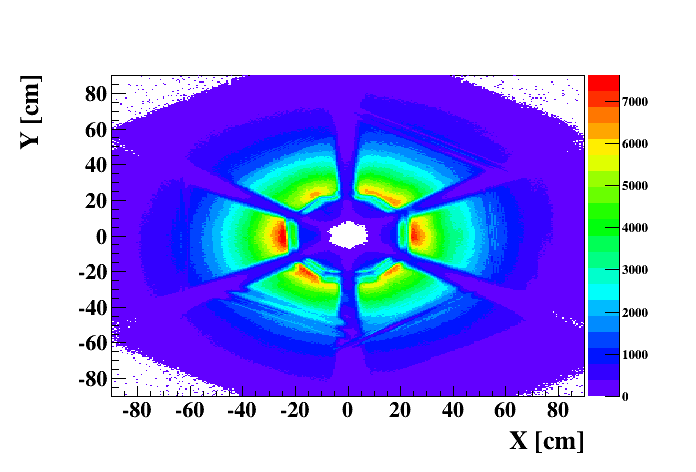
\includegraphics[scale=0.35]{fig_analysis/proton_DC_IC_XY_1.png}
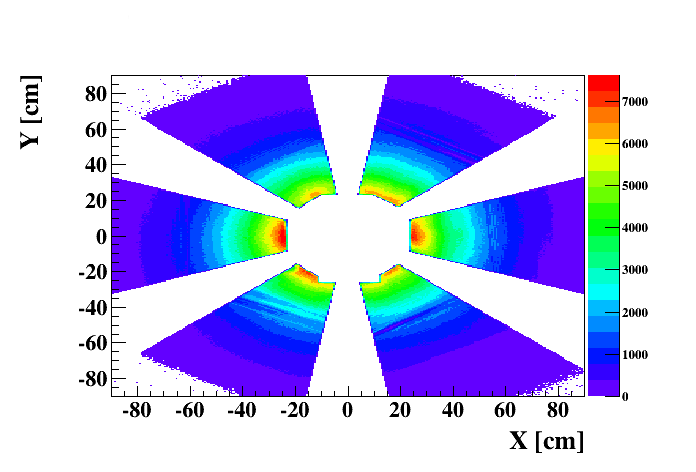
\includegraphics[scale=0.35]{fig_analysis/proton_DC_IC_XY_3.png}
\caption{XY plane projection in DC1 for the positive particles before (left) and after (right) IC shadow and DC fiducial cuts.} 
\label{fig:proton_DC_IC_cut}
\end{figure}
 
\item Velocity ($\Delta \beta$) cut: the previous cuts do not separate the protons from other positive particles, such as positive pions and kaons. A very clear separation can be obtained by associating the information from the SCs and the DCs. The velocity of a charged particle can be calculated by using the momentum ($p$) reconstructed in the DCs and the Time-Of-Flight ($t_{TOF}$) measured by the SCs. We define:
\begin{equation}
\Delta \beta = \beta_{SC} - \beta_{DC} = \frac{l_{track}}{c \cdot t_{TOF}} - \frac{p}{\sqrt{p^{2} + m^{2}_{p}}}~,
\end{equation}
where $l_{track}$ is the measured track length and $m_{p}$ is the proton mass. On the left plot of figure \ref{fig:proton_delta_beta_cuts}, $\Delta \beta$ is plotted as function of momentum. One can see two main trends in this plot: the region around zero corresponds to the protons, while the one above corresponds to the positive pions ($\pi^{+}$). The right plot shows a one-dimensional distribution of $\Delta \beta$ zoomed in the region of the protons.
\begin{figure}[tbp]
\hspace{-0.2in}
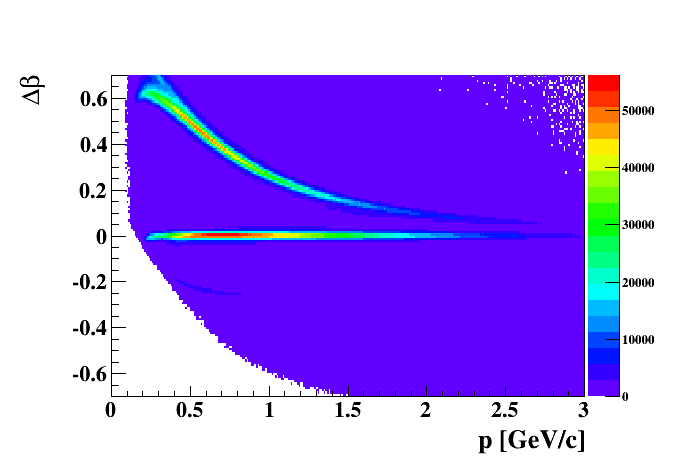
\includegraphics[scale=0.36]{fig_analysis/prot_DeltaBeta_p.png}
\hspace{-0.2in}
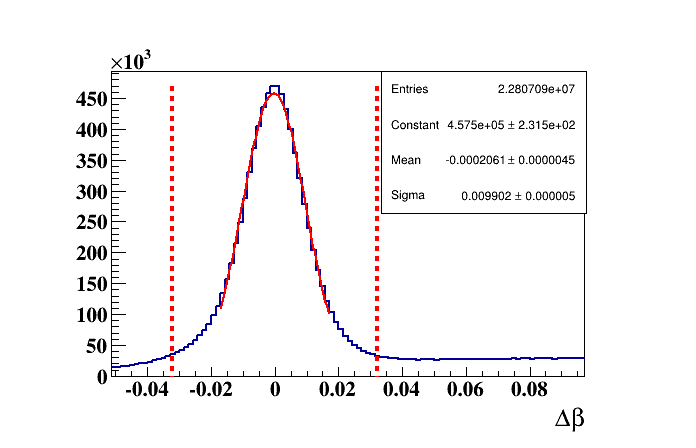
\includegraphics[scale=0.36]{fig_analysis/prot_DeltaBeta.png}
\caption{On the left: $\Delta \beta$ as a function of $p$ for the detected positive particles after the fiducial cuts. On the right: one-dimensional distribution of $\Delta \beta$ zoomed in the region of the protons. The red dashed lines represent $\pm$3$\sigma$ cuts around the mean to select good reconstructed protons.} 
\label{fig:proton_delta_beta_cuts}
\end{figure}

\item Vertex matching:  the last cut is the correspondence between the longitudinal vertices of the detected electron and proton. Figure \ref{fig:proton_delta_z_e_prot} shows the difference $\Delta z = z_{e} - z_{p}$ and the chosen cuts (red dashed lines).
\end{itemize}
~~~~Finally, figure \ref{fig:prot_Theta_Phi} shows the azimuthal angle as a function of the polar angle distribution for the identified protons after all the selection cuts. One notices that the population of the protons is different from one sector to another, which comes from the dead regions in some sectors.
\vspace{-0.1in}
 
\begin{figure}[tbp]
\begin{minipage}[c]{.46\linewidth}
\hspace{-0.3in}
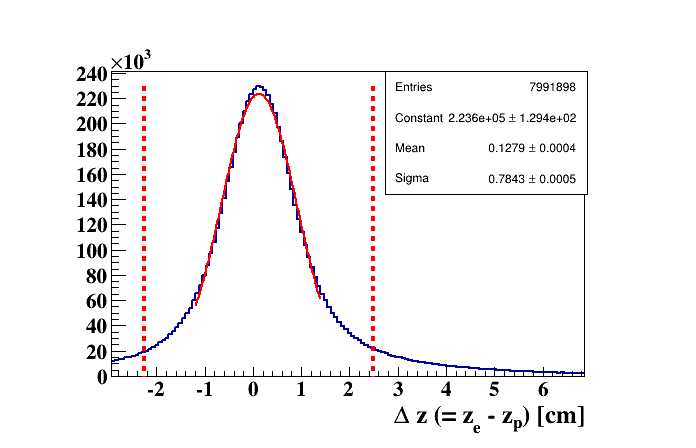
\includegraphics[height=6.0cm]{fig_analysis/proton_delta_z_e_prot.png}
\caption{$\Delta z$ distribution. The red dashed lines indicate $\pm$3$\sigma$ cuts around the mean. } 
\label{fig:proton_delta_z_e_prot}
\end{minipage} \hfill
\begin{minipage}[c]{.46\linewidth}
\hspace{-0.3in}
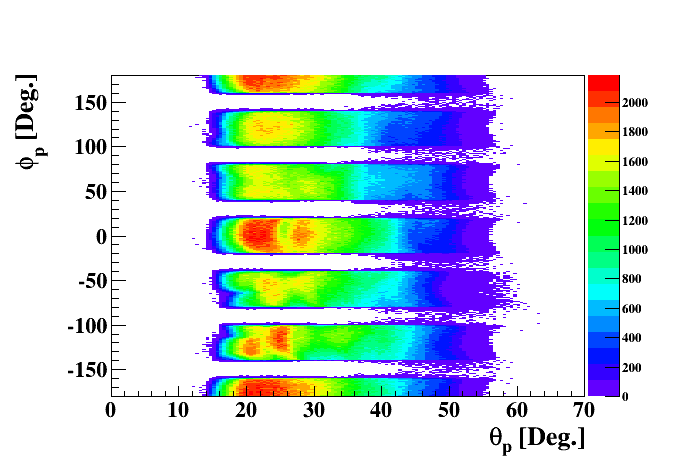
\includegraphics[height=6.0cm]{fig_analysis/prot_Theta_Phi_2.png}
\caption{$\phi$ vs. $\theta$ for the selected protons.}
\vspace{0.2in}
\label{fig:prot_Theta_Phi}
\end{minipage}
\end{figure}

\subsection{Photon identification}
~~~~CLAS is equipped with two calorimeters that can detect photons: the IC, covering polar angles from 4$^\circ$ to 14$^\circ$, and the EC, covering polar angles from 8$^\circ$ to 45$^\circ$. Like for the other particles, in addition to the coincidence with one good electron, we require a set of criteria to ensure the quality of the detected photons. Due to the efficiency constraints in both calorimeters, we restrict the energy of the selected photons to be greater than 300 MeV. Further requirements are applied depending on each detector.   

\subsubsection*{EC photons}
A particle has to pass the following conditions in order to be considered a good photon: 

\begin{itemize}
\item Neutral charge: this condition is achievable via the information from the drift chambers. A photon candidate in the EC must not be associated with a track in the DCs.

\item EC fiducial cut:  like for the electrons, this requirement is made to reject the photons which are detected at the edges of the EC. Figure \ref{fig:photons_EC_XY_photon_2.png} shows the XY plane distribution of EC neutral particles. We use the cuts: 100 cm < $U$, $V$ < 360 cm, and $W$ < 390 cm, to select the EC photons.

\item Velocity ($\beta$) cut: the scattered electron and its associated photon originate from the same vertex. Knowing the electron vertex ($\overrightarrow{V_{e}}$) and the photon hit position in the EC ($\overrightarrow{R_{\gamma}}$), one can calculate the photon velocity $\beta$ as:
\begin{equation}
\beta_{\gamma} = \frac{l}{ct} = \frac{|\overrightarrow{R_{\gamma}} - \overrightarrow{V_{e}}|}{c (t_{EC} - t_{trg})}
\end{equation}
where $l$ is the traveled distance from the vertex to the hit point in the EC. The traveling time ($t$) is calculable from the relative difference between the trigger time ($t_{trg}$) and the EC timing ($t_{EC}$). Figure \ref{fig:photons_beta_EC} shows the $\beta$ distribution of the neutral particles in the EC.
\end{itemize}
\begin{figure}[tp]
\begin{minipage}[c]{.46\linewidth}
\hspace{-0.3in}
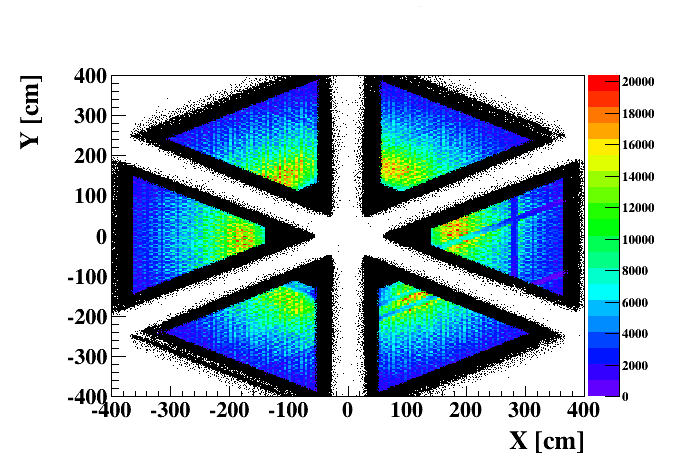
\includegraphics[height=6.0cm]{fig_analysis/photons_EC_XY_photon_2.png}
\caption{XY projection of the neutral particles in the EC. The coloured regions represent photons which passed the EC fiducial cuts, while the black regions are out of the fiducial cuts.} 
\label{fig:photons_EC_XY_photon_2.png}
\end{minipage} \hfill
\begin{minipage}[c]{.46\linewidth}
\hspace{-0.5in}
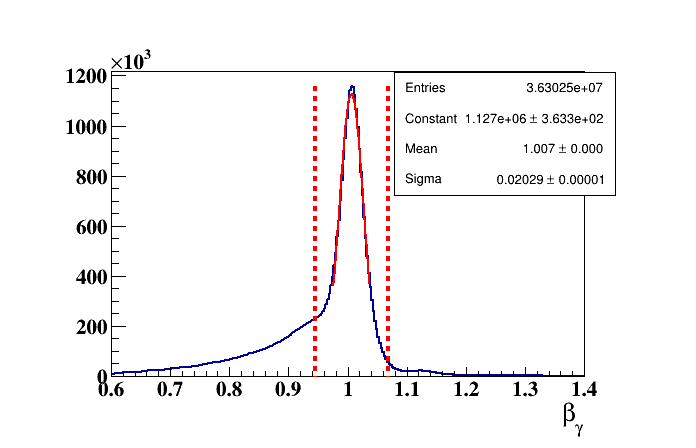
\includegraphics[height=6.0cm]{fig_analysis/photons_beta_EC.png}
\caption{$\beta$ distribution of neutral particles in the EC. The two vertical lines represent $\pm$3$\sigma$ cuts around $\beta$~=~1 to select photons.}
\vspace{+0.3in}
\label{fig:photons_beta_EC}
\end{minipage}
\end{figure}



\subsubsection*{IC photons}
For IC photons, we use the following cuts:
\begin{itemize}
\item IC fiducial cuts: the photons which hit the edges of the IC deposit only 
   part of their energies within the calorimeter. For this reason, we reject 
   the photons which hit the innermost or the outermost rings of the IC.  
   Figure \ref{fig:photons_IC_XY_2} illustrates this cut \cite{FX_thesis}.
\item M\o ller electrons reduction: a two-dimensional plot of photon polar 
   angles as a function of the energy shows an overcrowded region at low 
   $\theta$ and low energy. This can be seen in figure 
   \ref{fig:photons_IC_theta_En_1}. This region is mostly populated by the M\o 
   ller electrons and must be excluded from the analysis. We optimized a linear 
   cut for this region, shown by the black dashed line. The vertical extension 
   of this line shows the minimum energy cut ($E_{\gamma}$ > 300 MeV).
\item We do not apply any timing cut to select the photons in the IC because 
   its timing is not functioning properly for certain channels. Therefore, 
   applying a timing cut would add inefficient regions in the detector that we 
   wanted to avoid.  Therefore, we rely mainly on exclusivity cuts to remove 
   any potential contamination.

\end{itemize}
\begin{figure}[tbp]
\begin{minipage}[c]{.46\linewidth}
\hspace{-0.4in}
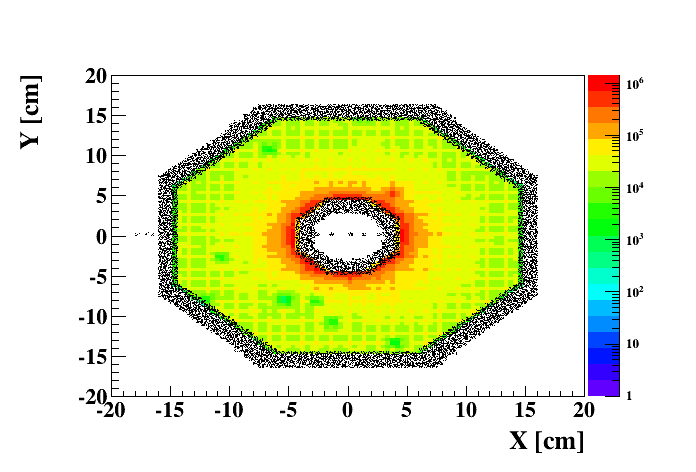
\includegraphics[height=6.0cm]{fig_analysis/photons_IC_XY_2.png}
\caption{XY distribution for the IC photons. The photons which hit the black innermost and outer regions are excluded from this analysis.} 
\label{fig:photons_IC_XY_2}
\end{minipage} \hfill
\begin{minipage}[c]{.46\linewidth}
\hspace{-0.4in}
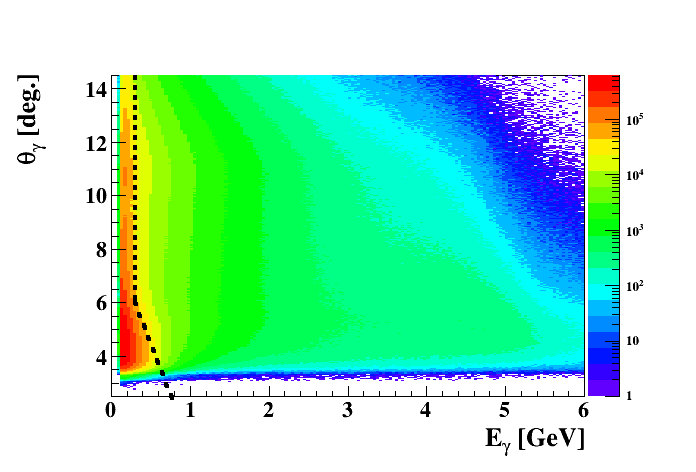
\includegraphics[height=6.0cm]{fig_analysis/photons_IC_theta_En_1.png}
\caption{$\theta$ versus $E$ for the IC photons which passed the fiducial cuts. The black dashed line represents the cut to reject the M\o ller electrons.}
\label{fig:photons_IC_theta_En_1}
\end{minipage}
\end{figure}
To summarize the photon selection, the two-dimensional distribution of azimuthal angle as a function of polar angle for IC and EC photons is shown in figure \ref{fig:photon_phi_theta}. 
\begin{figure}[tbp]
\hspace{-0.2in}
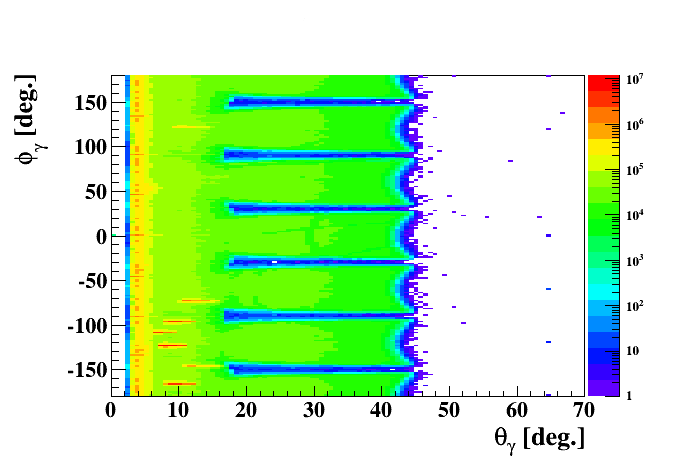
\includegraphics[scale=0.35]{fig_analysis/photon_phi_theta_1.png}
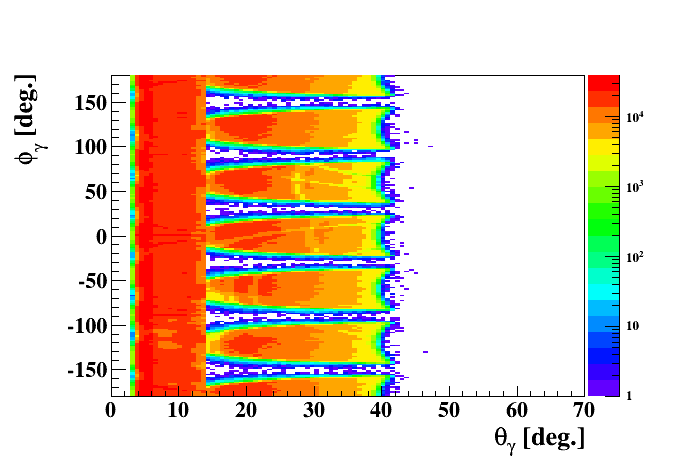
\includegraphics[scale=0.35]{fig_analysis/photon_phi_theta_2.png}
\caption{On the left: $\phi$ versus $\theta$ for all the neutral particles before the cuts. On the right: $\phi$ vs. $\theta$ for the the selected photons.} 
\label{fig:photon_phi_theta}
\end{figure}

\subsection{Helium-4 identification}
~~~~Details on the RTPC's structure and the definition of the different 
variables were given in chapter 2, section 2. In the following, we show the 
cuts to select the RTPC good tracks with a 6-GeV beam energy. The distributions 
will be shown for the two independent modules of the RTPC separately, labelled 
as left and right sides. The cuts are:

\begin{itemize}
\item Coincidence with one and only one good electron.  
\item Number of active pads greater than 3: the track has to have recorded hits 
   from at least four different readout pads. Figure \ref{fig:padnb} shows the 
   distribution of the number of active pads as a function of the total 
   momentum measured in the RTPC for the identified good tracks using 6 GeV 
   electron beam energy.
   
   \begin{figure}[tbp]
      \centering
      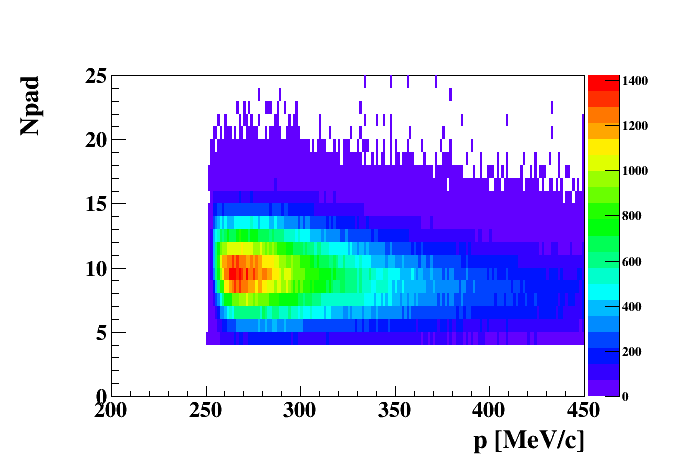
\includegraphics[height=7.2cm]{fig_analysis/npd_p.png}
      \caption{The number of active pads versus the measured p for the good 
      tracks collected using 6 GeV electron beam energy.}
      \label{fig:padnb}
   \end{figure}

\item Positive radius of curvature. 

\item Vertex cut: figure \ref{fig:rtpc_z} shows the z-vertices of the 
   positive-curvature tracks.

\item Track helix-fit quality: figure \ref{fig:rtpc_X2} shows the $\chi^{2}$ 
   distributions for the positive tracks originating within the RTPC. We apply 
   $\chi^{2}$~<~3.5 to select good $^4$He tracks.

\item $sdist$ and $edist$ cuts: figures \ref{fig:rtpc_sdist} and \ref{fig:rtpc_edist} show the $sdist$ and $edist$ distributions, for the positive tracks, originated within the RTPC, and having good $\chi^{2}$ values.

\item Z-vertex cut: like for the protons, the RTPC's reconstructed track has to originate from the same electron vertex. Figure \ref{fig:rtpc_delta_z} shows the difference between the $z$ of the reconstructed vertices of the electron and the associated RTPC tracks. 

\item Fiducial cuts: Figure \ref{fig:rtpc_phi_theta} illustrates the effect of 
   the fiducial cuts we apply on the azimuthal angles. 

\begin{figure}[tbp]
\begin{minipage}[c]{.46\linewidth}
\hspace{-0.3in}
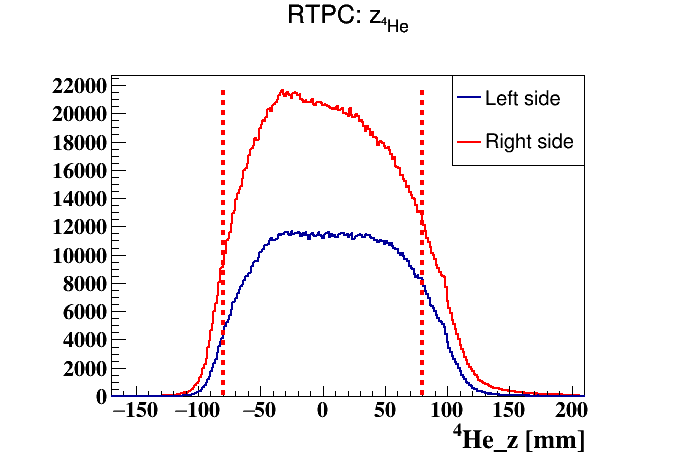
\includegraphics[height=6.0cm]{fig_analysis/rtpc_z.png}
\caption{ $z$-vertices for the reconstructed positive tracks with respect to 
the RTPC center (-64 cm with respect to the CLAS center), in the two modules of 
the RTPC. We chose the cut -80  mm < z < 80 mm to select good tracks.} 
\label{fig:rtpc_z}
\end{minipage} \hfill
\begin{minipage}[c]{.46\linewidth}
\hspace{-0.3in}
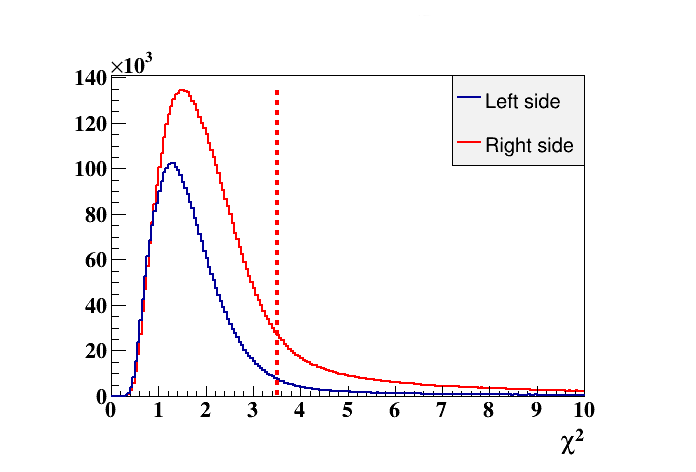
\includegraphics[height=6.0cm]{fig_analysis/rtpc_X2.png}
\caption{$\chi^{2}$ distribution for the tracks in the two modules of the RTPC, with the cut we require to select good tracks: $\chi^{2}$ < 3.5.}
\vspace{0.5in}
\label{fig:rtpc_X2}
\end{minipage}
\end{figure}

\begin{figure}[tbp]
\vspace{-0.3in}
\begin{minipage}[c]{.46\linewidth}
\hspace{-0.3in}
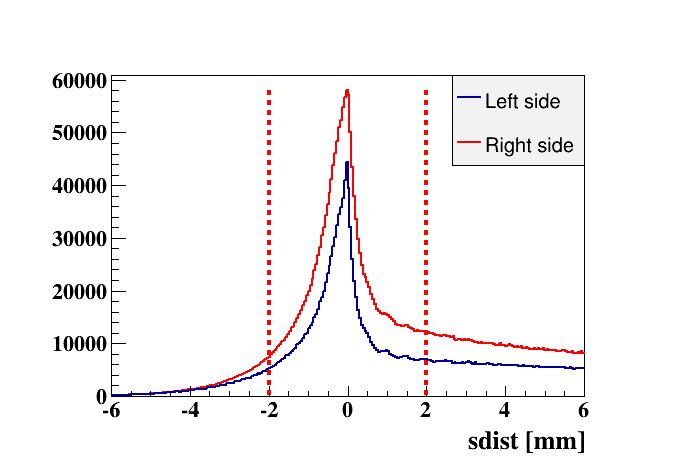
\includegraphics[height=6.0cm]{fig_analysis/rtpc_sdist.png}
\caption{$sdist$ distribution for the positive tracks in the RTPC. $|sdist|$~<~2.0 mm cut is applied to select good tracks.} 
\label{fig:rtpc_sdist}
\end{minipage} \hfill
\begin{minipage}[c]{.46\linewidth}
\hspace{-0.3in}
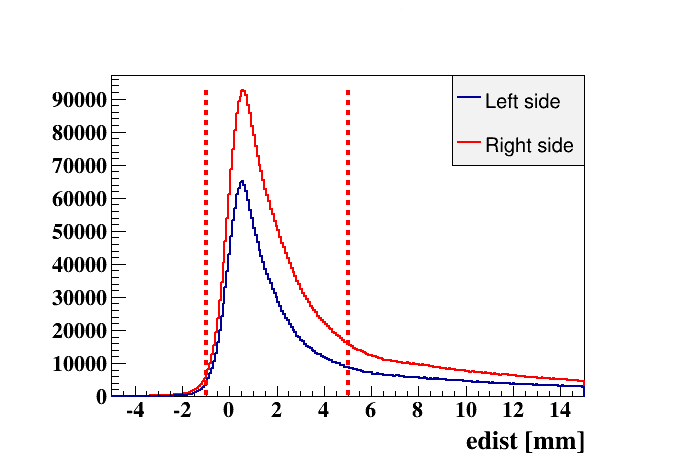
\includegraphics[height=6.0cm]{fig_analysis/rtpc_edist.png}
\caption{$edist$ distribution for the positive tracks in the RTPC. We require $-1.0$~mm~<~$edist$~<~5.0 mm to select good tracks.}
\label{fig:rtpc_edist}
\end{minipage}
\end{figure}

\begin{figure}[tbp]
\centering
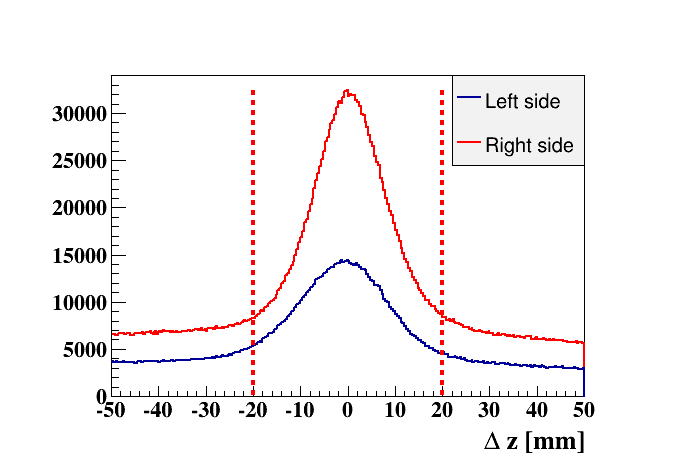
\includegraphics[scale=0.4]{fig_analysis/rtpc_delta_z.png}
\caption{The correspondence between the z-vertices of the detected electron and 
the good track in the RTPC. We require the absolute value of $\Delta z$ to be 
less than 20 mm.} \label{fig:rtpc_delta_z}
\end{figure}

\item In this work, due to the wide bands in dEdx distributions, we do not use 
   this quantity to select the recoil $^{4}He$ nuclei. We claim that the 
   kinematic exclusivity cuts, that are presented in chapter 4, are sufficient 
   to select coherent $^{4}He$ DVCS events. A systematic check about this question
   is presented in chapter 4.  


\end{itemize}

\begin{figure}[tbp]
\hspace{-0.2in}
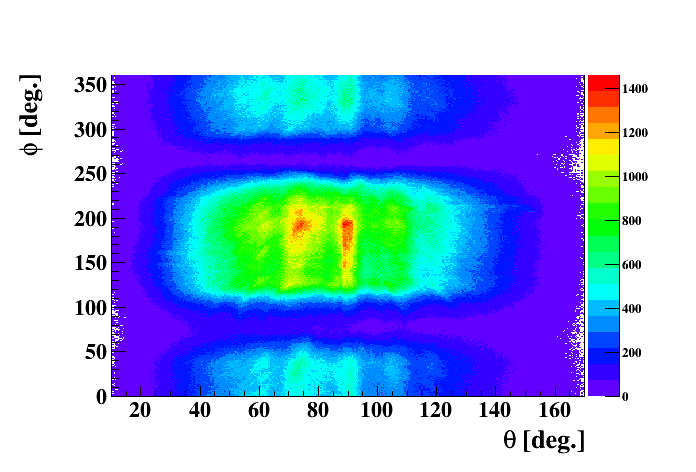
\includegraphics[scale=0.35]{fig_analysis/rtpc_phi_theta_1.png}
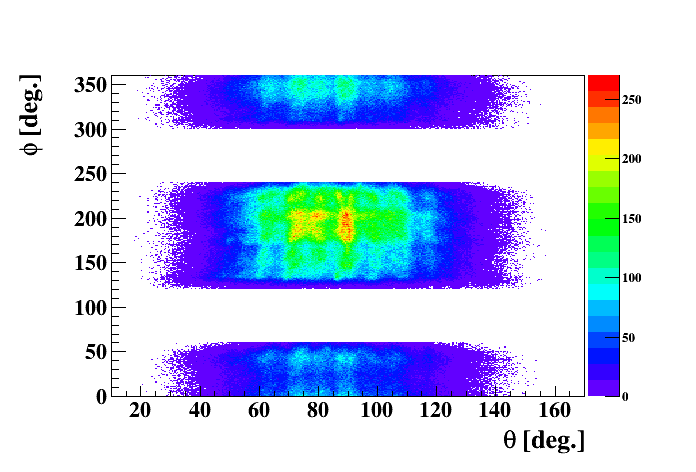
\includegraphics[scale=0.35]{fig_analysis/rtpc_phi_theta_2.png}
\caption{On the left: $\phi$ vs. $\theta$ for the positive-curvature tacks in the RTPC before the cuts. On the right: the same distribution after all the cuts.} 
\label{fig:rtpc_phi_theta}
\end{figure}

\subsection{$\pi^{0}$ identification}
~~~~In this analysis, we identify the $\pi^{0}$s with the goal of DVCS background subtraction as will be addressed in section \ref{Background_subtraction}. The $\pi^{0}$ identification is based on its two real photons decay mode ($\pi^{0} \rightarrow \gamma \gamma$), with a branching ratio around 98.8$\%$. In our experimental configuration, the reconstructed neutral pions can be categorized into three topologies: ICIC (the two photons are detected in the IC), ICEC (one photon in the IC and the second in the EC), and ECEC (the two photons are detected in the EC). The nominal mass of the $\pi^{0}$ is 0.135 GeV/c$^{2}$. The reconstructed invariant mass of the detected pair of photons can be seen in figure \ref{fig:pi0_selection}, for the three topologies. One can see clear peaks corresponding to the neutral pions in the three distributions.
\begin{figure}[tbp]
\hspace{-0.2in}
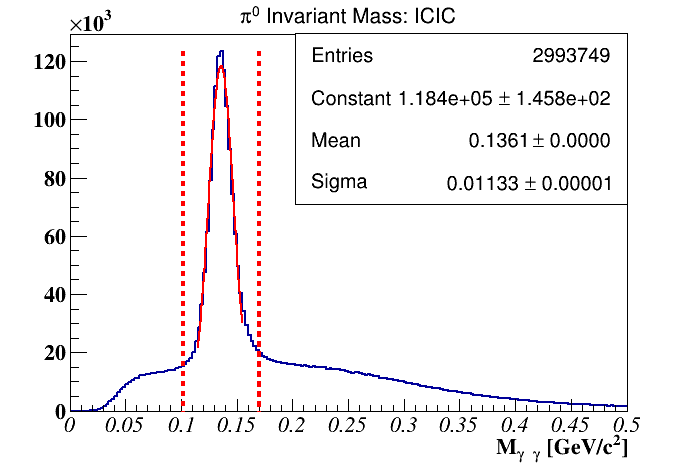
\includegraphics[scale=0.34]{fig_analysis/m_pi0_icic.png}
\hspace{-0.2in}
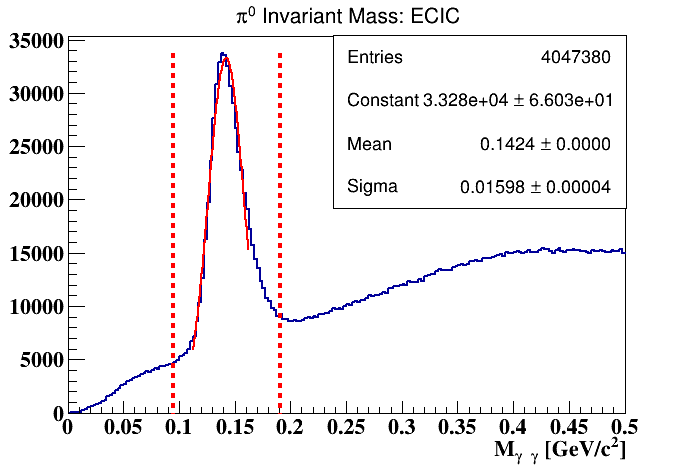
\includegraphics[scale=0.34]{fig_analysis/m_pi0_ecic.png}
\hspace*{-0.1in}
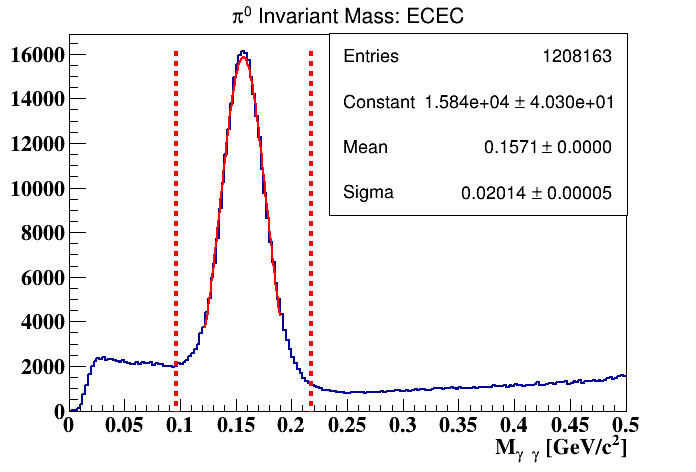
\includegraphics[scale=0.34]{fig_analysis/m_pi0_ecec.png}
\hspace{-0.2in}
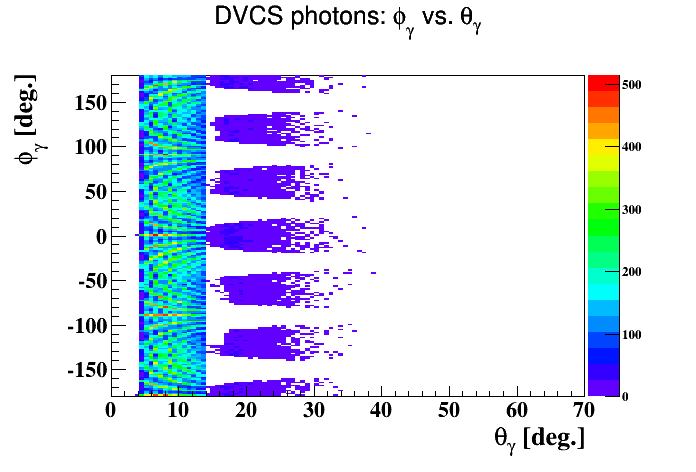
\includegraphics[scale=0.38]{fig_analysis/sim_photon_phi_theta_2.png}
\caption{The reconstructed invariant mass of the photon pairs in the three topologies: ICIC, ECIC and ECEC. On the bottom-right: $\phi$ vs. $\theta$ distribution for the simulated DVCS photons, shown that most of the DVCS photons are located in the IC.} 
\label{fig:pi0_selection}
\end{figure}\\

One can conclude from the mean and sigma values of the distributions in figure \ref{fig:pi0_selection} that the IC has a better energy resolution than the EC. About 97$\%$ of the simulated DVCS events, as can be seen in the bottom-right plot, have the real photon emitted at very forward angles covered by IC. For these reasons, we chose to exclude the DVCS events which have their photons in the EC. Hence we are left with the two $\pi^{0}$ topologies, ICIC and ICEC, for the background subtraction as will be addressed later in this chapter.


\section{Simulation}
~~~~The Monte-Carlo simulation is used in this analysis for two goals: understanding the behaviour of the particles of interest in the detectors, and computing the acceptance for the DVCS background subtraction. The key stages of the simulation are summarized in figure \ref{fig:simulation_steps}: Monte-Carlo generated events pass in a GEANT3 simulation (GSIM) for the CLAS detector, then are processed with a package called GPP to add resolution and efficiency effects, and finally are reconstructed by a package named RECSIS, from which we obtain the physical quantities of each particle, like it is done for real data. In the following, each simulation stage will be briefly presented.
\begin{figure}[tbp]
\centering
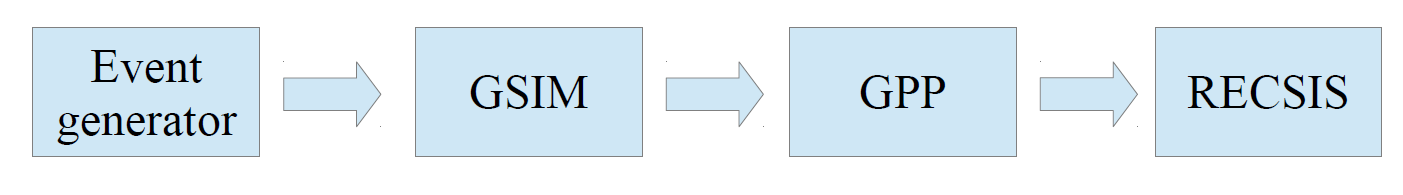
\includegraphics[scale=0.25]{fig_simulation/simulation_steps.png}
\caption{ The scheme shows the main simulation steps.} 
\label{fig:simulation_steps}
\end{figure}

\subsection{Event generator} \label{Event_generator}
~~~~Events are generated in the measured ranges of $Q^{2}$, $x_{B}$, $t$, and 
$\phi$ following a parametrization of the cross section which roughly 
reproduces the DVCS and exclusive $\pi^{0}$ electroproduction data 
\cite{FX_thesis}:
\begin{equation}
\frac{d^{4}\sigma}{dQ^{2}dx_{B}dtd\phi} \propto \left(\frac{Q^{2}_{0}}{Q^{2}}\right)^{\alpha} *  \frac{1}{1 + (\frac{x_{B} - x_{c}}{c})^{2}} * \frac{1}{(1+bt)^{\beta}} * (1-d(1-cos(\phi)).
\label{equ:event_generator}
\end{equation}
This parametrization is the product of four factors which reproduce the DVCS and $\pi^{0}$,  characteristics as follows:
\begin{itemize}
\item the $Q^{2}$-dependent term accounts for the depth of the interaction: $Q^{2}_{0}$ is the minimum allowed value and the $\alpha$ is a parameter which controls the shape of the distribution.   
\item the $x_{B}$ term accounts for the dependence of the cross section on the parton distribution functions, with $x_{c}$ the mean value of the Bjorken variable $x_{B}$.
\item the $t$ term accounts for the t-dependence of the elastic form factors of the helium and of the proton, via the parameters $b$ and $\beta$.
\item the $\phi$ term accounts for the cross section dependence on this angle, via the parameter $d$. The DVCS and the BH have a different behaviour than the $\pi^{0}$ exclusive events. 
\end{itemize}

~~~~Table \ref{Table:event_generator_values} shows the values of the parameters used for the cross section parametrization of the four channels of interest: $e^{4}He\gamma$, $e^{4}He\pi^{0}$, $ep\gamma$, and $ep\pi^{0}$.

\begin {table}[tbp]
\begin{center}
\begin{tabular}{|l|l|l|l|l|}
\hline
Parameter & $e^{4}He\gamma$  & $e^{4}He\pi^{0}$ & $ep\gamma$  & $ep\pi^{0}$ \\
\hline
$Q^{2}_{0}$ & 1.0 $GeV^{2}$/c$^{2}$ & 1.0 $GeV^{2}$/c$^{2}$ & 1.0 $GeV^{2}$/c$^{2}$ & 1.0 $GeV^{2}$/c$^{2}$ \\
\hline
$\alpha$ & 2.5 & 3.0 & 1.5 & 1.5 \\
\hline
b & -11.0 $GeV^{2}$/c$^{2}$ & -8.8 $GeV^{2}$/c$^{2}$ & -1.408 $GeV^{2}$/c$^{2}$& -1.408 $GeV^{2}$/c$^{2}$\\
\hline
$\beta$ & 12.0 & 7.3 & 4.0 & 1.5\\
\hline
$x_{c}$ & 0.2 & 0.3 & 0.2 & 0.5\\
\hline
c & 0.2 & 0.3 & 0.2 & 0.5 \\
\hline
d & 0.4 & 0 & 0.4 & 0 \\
\hline
\end{tabular}
\caption{ Values of the parameters adapted in our event generator.}
\label{Table:event_generator_values}
\end{center}
\end{table}

~~~~Regarding the protons in $ep\gamma$ and $ep\pi^{0}$ channels, we apply the 
Fermi motion on the initial protons based on the parametrization of C. Ciofi 
degli Atii and S. Simula \cite{fermi_motion}. Figure \ref{fig:fermi_mom} shows 
the Fermi momentum distributions of the nucleons inside $^{4}He$, where we 
apply a cut on the high-momentum tail at 0.3 GeV/c, higher momentum should not 
contribute to the final DVCS sample because of our exclusive cuts presented in 
the following chapter. 

\begin{figure}[tbp]
\centering
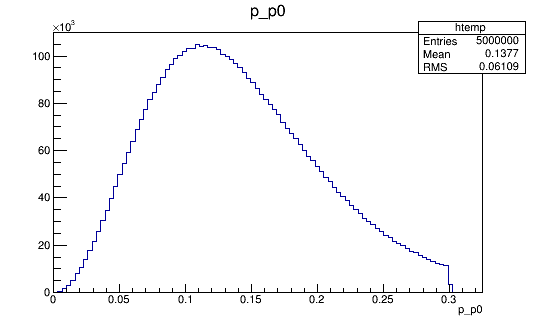
\includegraphics[scale=.55]{fig_analysis/fermi_momentum_dis.png}
\caption{ Fermi momentum distribution of the nucleons inside $^{4}He$, in 
$GeV/c$.} \label{fig:fermi_mom}
\end{figure}



\subsection{GSIM}
~~~~GSIM is a GEANT3-based simulation of the CLAS detector, developed by the CLAS collaboration \cite{GSIM}. This simulation takes into account all the experimental environment, such as the target's position, materials, and geometry, and also the various sub-detectors' materials and geometries, to reproduce the behaviour of particles traversing the detector. {\it Nota Bene} the reconstruction in the RTPC is not implemented in GSIM, however its material is present.

\subsection{GPP}
~~~~For the purpose of making the simulation more realistic, the output of GSIM is fed to the GSIM Post-Processing (GPP) package. This package applies resolution effects on the different measured quantities, and also reads efficiency maps to match the simulation to the real experiment. The resolutions are categorized into three groups, time, position, and energy resolution. In the following, we present the techniques used in this work to extract the smearing factors for the simulation.

\paragraph{SC time smearing}
~\\
~\\
~~~~The GPP takes a single factor to smear the time in a Gaussian form. Figure \ref{fig:SC_smearing_factors} shows an illustration of the time smearing effects, in which $\Delta \beta$ for the protons \\($\Delta \beta~=~\beta_{measured}~-~\beta_{calculated}$~) is compared for data and simulation. The chosen SC smearing factor is 2.1.

\paragraph{DCs position smearing}
~\\
~\\
~~~~The GPP uses three factors to smear the positions of the hits in the DCs, in a Gaussian form. These smearing factors are extracted from comparing simulation to data in terms of the Time-Based Tracking (TBT) residual distributions, i.e. the deviation of the hits in the DCs from the fitted track. Figure \ref{fig:DC_smearing_factors} shows the experimental, initial simulated, and smeared simulated residual distributions for the collected good electrons and protons. The extracted smearing factors are: ($a$, $b$, $c$) = (1.1, 0.85, 1.1), where the factor $a$ stands for smearing of DC1, $b$ for DC2, and $c$ for DC3. One can see the smearing effects by looking to the values of $\sigma$ from the fit in each Super-Layer (SL). We conclude that these factors match the simulation to the data.
\begin{figure}[tbp]
\hspace{-0.7in}
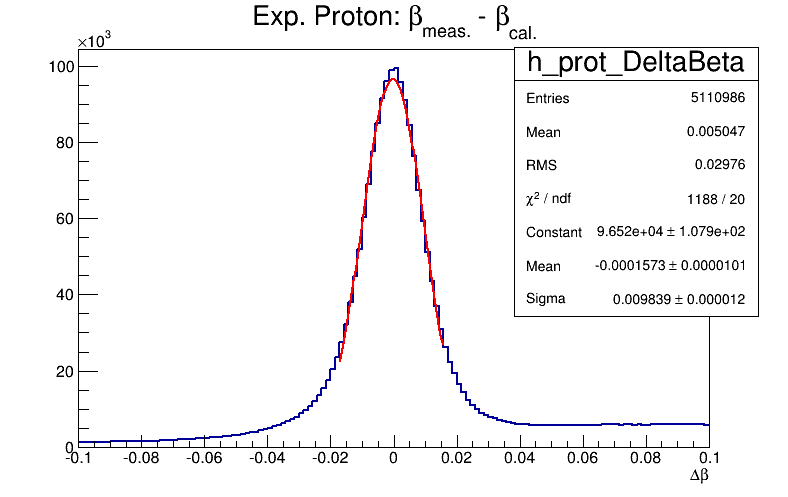
\includegraphics[scale=0.3]{fig_simulation/Exp_proton_delta_beta.png}
\hspace{-0.1in}
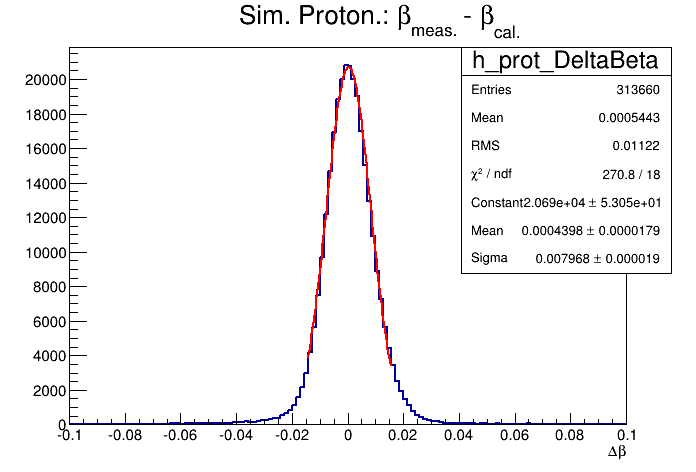
\includegraphics[scale=0.32]{fig_simulation/Sim_proton_delta_beta.png}
\centering
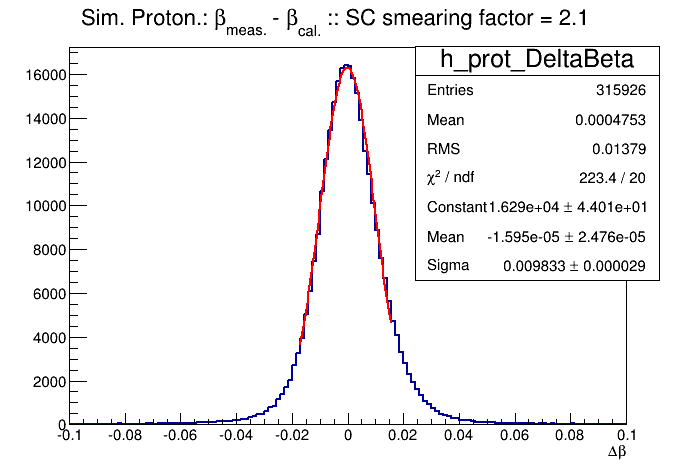
\includegraphics[scale=0.32]{fig_simulation/Sim_proton_delta_beta_smeared.png}
\caption{Illustration of the SC time smearing via the $\Delta \beta$ distributions for the protons. On the top left: $\Delta \beta$ distribution of the experimental data. On the top right: the simulated data without smearing. On the bottom: the simulated data after SC time smearing with a factor equal to 2.1.} 
\label{fig:SC_smearing_factors}
\end{figure}

\begin{figure}[tbp]
\centering
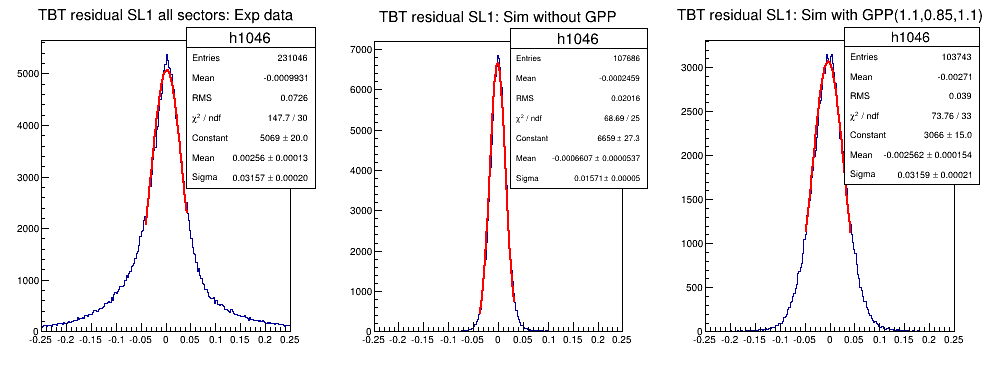
\includegraphics[scale=0.47]{fig_simulation/Ele_SL1.png}
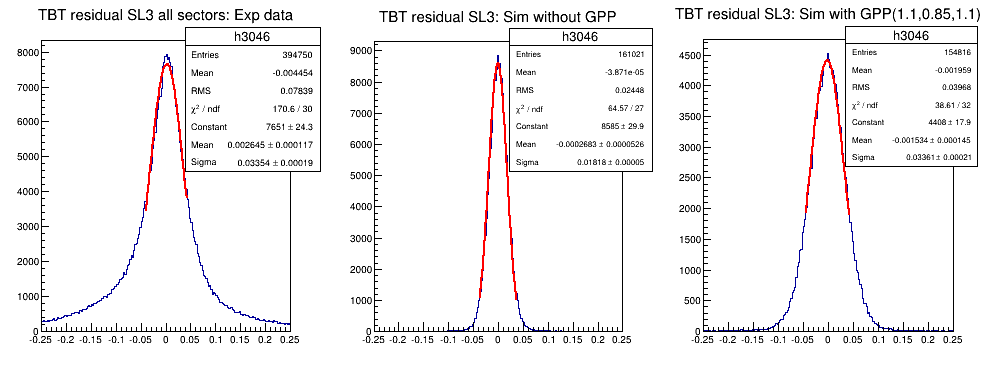
\includegraphics[scale=0.47]{fig_simulation/Ele_SL3.png}
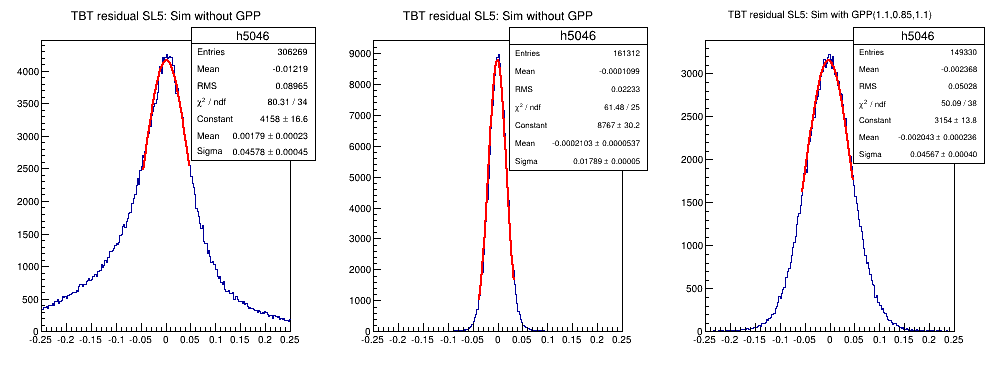
\includegraphics[scale=0.47]{fig_simulation/Ele_SL5.png}
\caption{Time-Based Tracking (TBT) residual distributions for the electrons and the protons in the first super-layer (top panel), the second super-layer (middle panel) and the third super-layer (bottom panel) of the experimental data (first column), of the simulation without GPP (second column), and the simulation with GPP DC-position smearing factors: 1.1, 0.85, and 1.1 for $a$, $b$, and $c$ respectively. } 
\label{fig:DC_smearing_factors}
\end{figure}


\paragraph{IC energy smearing}
~\\
~\\
~~~~An energy smearing for the IC photons is also needed. The GPP software uses three factors to perform this smearing: $ic\_a$, $ic\_b$, and $ic\_c$, where $ic\_a$ accounts for the smearing of the width of the noise around zero using a Gaussian, while $ic\_b$ and $ic\_c$ are the smearing factors for the ADC values, using Gaussians as well. Our parameters are: 0.008, 0.036, and 0.024 respectively. Figure \ref{fig:IC_smearing_factors} shows the effect of these smearing factors on the simulated invariant mass of the $\pi^{0}$. The associated experimental distribution can be seen on the top left plot of figure \ref{fig:pi0_selection}. One notices that the smeared width of the simulated distribution matches the measured experimental one.\\

\begin{figure}[tp]
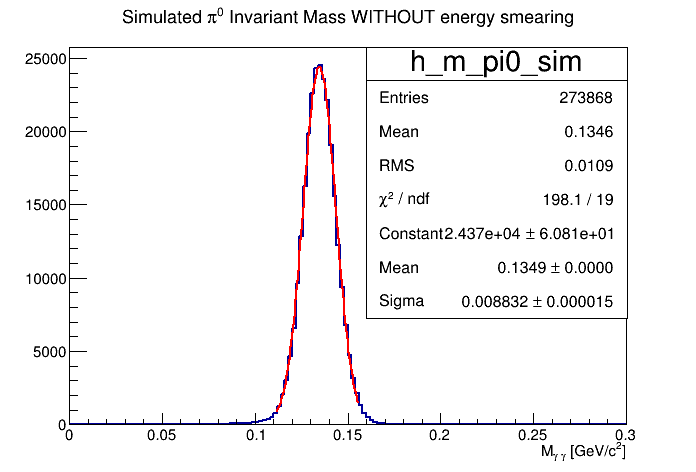
\includegraphics[scale=0.32]{fig_simulation/m_pi0_sim_without_smearing.png}
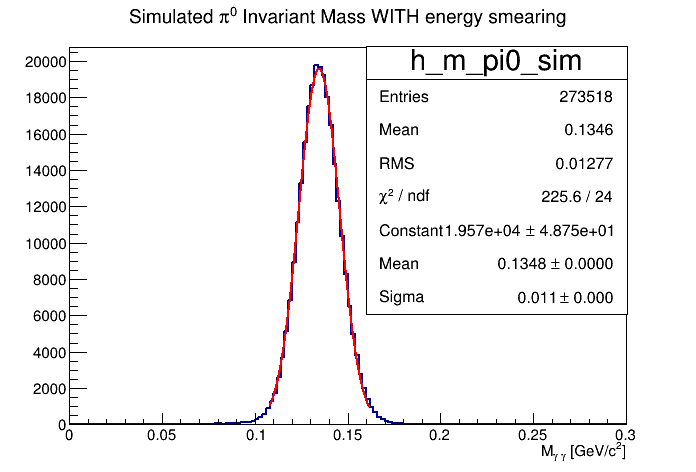
\includegraphics[scale=0.32]{fig_simulation/m_pi0_sim_with_smearing.png}
\caption{The invariant mass of the Monte-Carlo simulated $\pi^{0}$ without IC energy smearing, on the left, and with smearing, on the right. } 
\label{fig:IC_smearing_factors}
\end{figure}

\subsection{RECSIS}

~~~~RECSIS is the reconstruction package of CLAS which is used for both data 
and simulation. The detector responses, in terms of ADCs and TDCs, are 
converted by RECSIS into physical meaningful physical quantities, such as 
momentum, using lookup tables. In this process, the thresholds on the different 
detectors (DCs, CCs, ECs, SCs, IC, and RTPC) are applied to filter the signals 
before the reconstruction procedures. After this reconstruction, the outputs of 
RECSIS for the experimental and the simulated events can be compared directly, 
as will be presented in the next section.

\subsection{RTPC fastmc}
~~~~All the sub-detectors of CLAS are implemented in the GSIM GEANT3 simulation, 
however the RTPC is only there as dead material. As it is a more recent detector
it has been fully simulated using a stand alone GEANT4 simulation. As a 
first step, we replace this RTPC's simulation by a fast Monte-Carlo (fastmc) 
package at the level of the event generator to make the simulated $^{4}He$ more 
realistic and matching the data. This fastmc smears the $^{4}He$ kinematics and 
applies the RTPC's acceptance. Regarding the smearing, the momentum, polar 
angle, azimuthal angle and z-vertex of the $^{4}He$ are smeared with Gaussians 
using the observed tracking resolutions of the RTPC (see chapter 2, section 3).  
For the acceptance, the fastmc:
\begin{itemize}
\item ensures that the $^{4}He$ track intersects the cathode and the gems of the RTPC.
\item removes the tracks which pass in the dead area between the two modules of the RTPC.
\item removes the track if it goes to the upstream end of the target's holder.
\item applies the RTPC's thresholds on the momentum and the polar angle.
\end{itemize} 

The fastmc is applied to the Monte-Carlo generated $^{4}He$ for the channels 
$e^{4}He\gamma$ and $e^{4}He\pi^{0}$. We do not specifically apply energy loss 
and multiple scattering in our fastmc, but we do apply resolution effects based 
on experimental data that include both effects. The plots in figure 
\ref{fig:comp_He} show the comparison between data and simulation in terms of 
$\theta$, $\phi$ and momentum of the $^{4}$He DVCS nuclei, that will presented 
in details in the following chapter. The other particles, ($e^{-}$, $p$, 
$\gamma$), are fed to GSIM through the previously mentioned 
simulation-reconstruction chain procedures.

\begin{figure}[tpb]
   \includegraphics[height=5.0cm]{fig_rtpc/updates/He_theta.png}
   \includegraphics[height=5.0cm]{fig_rtpc/updates/He_phi.png}
   \centering
   \includegraphics[height=5.0cm]{fig_rtpc/updates/He_mom.png}
   \caption{Comparison between experimental (blue) and simulated (red) DVCS 
   $^{4}$He nuclei in terms of polar angle, azimuthal angle and momentum.}
   \label{fig:comp_He}
\end{figure}


\section{Kinematic Corrections}
~~~~~The simulation enables us to extract kinematic corrections for the different particles, by comparing the reconstructed physical quantities from the simulation to the initially generated ones. In general, the reconstructed azimuthal angles of all the particles are consistent with the generated ones, while the reconstructed polar angles and momenta show some deviations. Therefore, corrections are required. In the following, the electron and the proton corrections are applied on both data and simulation, while the simulated photons are corrected differently from the experimental ones, as will be explained and justified. 

\subsection{Electrons}
~~~~The reconstructed kinematics of the simulated electrons are roughly consistent with the generated quantities, as can be seen in figure \ref{fig:electron_corrections}. Nevertheless, we extracted and applied corrections on the electrons to achieve a higher precision. The corrected polar angles and momenta take the form:
\begin{equation}
\theta_{corr.} = \frac{\theta_{rec.}}{f(\theta_{rec.})} ~~~~~~~ p_{corr.} = \frac{p_{rec.}}{f(p_{rec.})}
\label{equation:correcting_function}
\end{equation}  
where $f(\theta_{Rec.})$ and $f(p_{Rec.})$ are the functions shown, respectively, on the left and right plots of figure \ref{fig:electron_corrections}.
\begin{figure}[tbp]
\centering
\includegraphics[scale=0.41]{fig_simulation/before_electron_Rec_gen.png}
\caption{Electron corrections. On the left: The ratio of the reconstructed to the generated electron polar angles is plotted as a function of the reconstructed polar angle. The mean of the distribution is parametrized by the black curve. On the right: the momentum ratio ($Rec/Gen$) is plotted as a function of the reconstructed momentum and parametrized by the black curve .} 
\label{fig:electron_corrections}
\end{figure}

\subsection{Protons}
~~~~The same procedures for the extraction of the kinematic corrections of the electrons have been carried out for the protons. The results can be seen in figure \ref{fig:proton_corrections}. The corrected polar angles and momenta are obtained using equations \ref{equation:correcting_function} and the functions shown on each plot of figure \ref{fig:proton_corrections}. 
\begin{figure}[tp]
\centering
\includegraphics[scale=0.41]{fig_simulation/before_proton_Rec_gen.png}
\caption{Proton corrections. On the left: the reconstructed-generated polar angle ratio is plotted as a function of the reconstructed angle and fitted with the black curve. On the right: the momentum ratio is plotted as a function of the reconstructed momentum.} 
\label{fig:proton_corrections}
\end{figure}


\subsection{IC photons in simulation} 
~~~~The simulated IC photons shows non-negligible polar angle and energy deviations from the expected kinematics. This can be seen in figure \ref{fig:simulated_ic_corrections}. These deviations are almost systematic shifts, in which the polar angle deviation might be coming from badly defined geometrical values within GSIM. For these photons, we followed the same techniques of comparing the reconstructed quantities to the generated ones in order to extract the correction functions.\\

\begin{figure}[tbp]
\centering
\includegraphics[scale=0.41]{fig_simulation/before_gamma_Rec_gen.png}
\caption{Corrections for the simulated IC photons. On the left: the reconstructed-generated polar angle's ratio is plotted as a function of the reconstructed polar angles. On the right: the energy ratio is plotted.} 
\label{fig:simulated_ic_corrections}
\end{figure}

As an illustration of the corrections, figure \ref{fig:egamma_difference} shows the squared $e\gamma X$ missing mass distribution for the simulated $ep\gamma$ DVCS events before the corrections, on the left, and after the corrections, on the right. In this configuration, the missing particle is the proton, such that the expected mean value should be the mass squared of the proton ($0.938^{2} = 0.8798$). The right value is obtained after the corrections.

\begin{figure}[tp]
\centering
\includegraphics[scale=0.32]{fig_simulation/egamma_MM2_before_corrections.png}
\includegraphics[scale=0.32]{fig_simulation/egamma_MM2_after_corrections.png}
\caption{An illustration of the corrections in terms of the squared $e\gamma X$ missing mass distribution for the $ep\gamma$ simulated DVCS events. } 
\label{fig:egamma_difference}
\end{figure}

\subsection{IC photons in real data} ~~~~For the experimental IC photons, we 
used the reconstructed invariant mass of the $\pi^{0}$ in the ICIC topology to 
ensure the consistency of the IC calibration over the acceptance of the detecor 
and the experimental running time. In this investigation, we require each 
$\pi^{0}$ photon to have a minimum energy of 500 MeV in order to avoid low 
efficiency effects of the IC. 

\subsubsection{Run-dependent energy correction}

In the CLAS-EG6 experiment, the reconstructed mass of the $\pi^{0}$ displays a linear dependence on the energy, as can be seen in figure \ref{fig:M_E_pi0_before_corrections}. In order to ensure the consistency of the calibration over time, we extracted this mass-energy dependence for the individual runs. Figure \ref{fig:ic_alpha_beta_fitting} shows the extracted slope ($\alpha$) and offset ($\beta$), from the linear fits of the mass versus the energy of $\pi^{0}$, as a function of run number. One notices a non-negligible variation over the experimental running period due to changes in the experimental conditions, such as changes in trigger requirements and beam position.\\

\begin{figure}[tbp]
\centering
\includegraphics[scale=0.25]{fig_simulation/M_E_pi0_before_corrections.png}
\caption{The invariant mass of the reconstructed $\pi^{0}$ as a function of its energy. The red line represents a linear fit.} 
\label{fig:M_E_pi0_before_corrections}
\end{figure}

\begin{figure}[tbp]
\centering
\includegraphics[scale=0.33]{fig_simulation/Alpha_RunNumber_before_corr.png}
\includegraphics[scale=0.33]{fig_simulation/Beta_RunNumber_before_corr.png}
\caption{The slope ($\alpha$) and the offset ($\beta$) from linear fits of M$_\pi^{0}$ vs. E$_\pi^{0}$, as a function of run number. The red lines represent the fitting functions.} 
\label{fig:ic_alpha_beta_fitting}
\end{figure}

 To extract energy corrections for IC photons, the two distributions of figure \ref{fig:ic_alpha_beta_fitting} have been parametrized by piecewise functions of the form:
\begin{equation}
\alpha (x) = c_{0} + c_{2} \left[ e^{-c_{3}(x - c_{1})} - e^{-c_{4}(x - c_{1})} \right],
\end{equation}
\begin{equation}
\beta (x) = p_{0} + p_{2} \left[ e^{-p_{3}(x - p_{1})} - e^{-p_{4}(x - p_{1})} \right],
\end{equation}
where the values of the parameters of $\alpha$ and $\beta$ can be found in Appendix \ref{App:AppendixA} (tables \ref{Table:ic_alpha_corrections} and \ref{Table:ic_beta_corrections} respectively). The requirement of a 500 MeV maximum difference between the two photons allows to assume that the two photons have approximately the same energy ($E_{\pi^{0}} = 2 E_{\gamma}$). Then, the correction take the form:
\begin{eqnarray}
\frac{E^{\pi^{0}}_{corr}}{M^{\pi^{0}}_{Theoretical} = 0.135 GeV} &=& \frac{E^{\pi^{0}}_{uncorr}}{M^{\pi^{0}}_{uncorr}}\\ 
\Longrightarrow
E^{\gamma}_{corr} &=& \frac{0.135*E^{\gamma}_{uncorr}}{\alpha(run)*2*E^{\gamma}_{uncorr} + \beta(run)}
\label{ic_corrrection_formula}
\end{eqnarray}
which takes as input the measured uncorrected photon energy ($E^{\gamma}_{uncorr}$), and the $\alpha$ and $\beta$ parameters, which depend on the run number. It then returns the corrected energy ($E^{\gamma}_{corr}$).\\

\subsubsection{Position correction}
~~~~Cluster position is reconstructed as a weighted average of its hits' positions.  Those hit positions are taken as the center of the front face of their corresponding crystal.  However, the energy deposition of the shower occurs at some depth into the crystal.  Due to the roughly focusing design of the calorimeter, this effect is negligible for photons originating from a vertex near the cystals' focal point.  However, for an extended target, and EG6 has the longest target used to date with this calorimeter, this effect is significant and a correction necessary.
%It is essentially a geometric projection effect.
%, and can be thought of as a coordinate transformation.

The focusing nature of this calorimeter allows us to treat this correction as only a shift in the radius of the cluster position, $\delta r$ (although other conventions could have been chosen, e.g.~only a shift in cluster $z$-position).  This is essentially a geometric projection effect, and it can be parameterized in terms of shower depth $d$, and the angle of the photon $\theta_\gamma$ with respect to that of the crystal's longitudinal axis, $\theta_C$:

\begin{equation}
  \delta r = \frac{d\sin(\theta_C-\theta_\gamma)}{\cos\theta_C}
  \label{eq:icDepthCorrection}
\end{equation}

Each photon's angle is calculated from its cluster's position ($x,y$) and the corresponding electron's $z$-vertex (or RTPC vertex in the case of EG6's neutral trigger).  The crystal angles are parameterized in terms of cluster position based on the calorimeter design drawings (where 78.3 cm is the focal length):

\begin{equation}
  \tan\theta_C=\frac{\sqrt{x^2+y^2}}{78.3\ \mathrm{cm}}
  \label{eq:cystalAngles}
\end{equation}

The shower depth parameter $d$ was treated as a free parameter and fit to the slope of $\sin(\theta_\gamma-\theta_C)$ versus $\cos\theta_C$, where $\delta r$ was determined by the PDG $\pi^0$ mass.  Energy-dependence of shower depth was investigated but empirically found to be insignificant.  The depth parameter was further tuned to minimize the $z$-dependence of the reconstructed $\pi^0$ mass peak, since $z$ is the most relevant reconstructed quantity least correlated with photon energy.

The resulting shower depth $d$ was estimated to be 5.56 cm in equation~\ref{eq:icDepthCorrection}.  The effect of this correction in terms of $z$-dependence is illustrated in figure~\ref{fig:ic_exp_correction_inv_mass_comp}.

\begin{figure}[tbp]
\centering
\includegraphics[width=8cm,height=6cm]{fig_analysis/NoDepthRunRadialE_finvMass_vz_pi0.png}
\includegraphics[width=8cm,height=6cm]{fig_analysis/NewDepthRunRadialE_finvMass_vz_pi0.png}
\caption{The measured fractional invariant mass of ICIC $\pi^{0}$ as a function of the electron $z$-vertex before (left) and after (right) cluster position corrections for shower depth.} 
\label{fig:ic_exp_correction_inv_mass_comp}
\end{figure}

\subsubsection{Radial-dependent energy correction}\label{sec:icraddepecorr}

After the previous corrections, we observed a remaining radial dependence of the reconstructed $\pi^{0}$ mass \cite{cristina}, where ``radial'' refers to the distance of the cluster from the beamline.  This can be seen in the left panel of figure \ref{fig:icRadiusEnergyData}.  
%We exhausted the possibilities of position corrections playing any role in this, and concluded this must be due 
This is most likely attributed to a systematic error in the original $\pi^0$-based gain calibration, which may not have fully accounted for correlations between crystals and the strong variation in rates with radius.  It is worth noting that this effect has also been observed in the eg1-dvcs experiment in $ep\gamma$ missing mass~\cite{eg1dvcs_photonenergy}.

\begin{figure}[tp]\centering
    \includegraphics[height=5.4cm]{fig_simulation/Mgg_radius_2plateau.png}
    \includegraphics[height=5.4cm]{fig_simulation/m_m0_pi0_radius_nathan.png}
    \caption{IC radial dependence of measured $\pi^0$ mass after all corrections prior to section~\ref{sec:icraddepecorr} (left).  Multidemesional dependence of $\pi^0$ mass on radius and energy for a subset of the data (right).\label{fig:icRadiusEnergyData}}
\end{figure}

To extract a correction for this behavior, photon pairs are selected with cluster radii differing by less than 1 cm and energies differing by less than 500 MeV.  Then the $\pi^0$ mass peak was fit in multidimensional bins of radius and energy.  The result was a clear linear dependence on energy within each radial bin; an example is shown in the right panel of figure~\ref{fig:icRadiusEnergyData}.  By fitting the linear energy-dependence for each radial bin, with results illustrated in figure~\ref{fig:icRadiusEnergySlopeOffset}, a correction function is derived:
\begin{equation}
E^{\gamma}_{final} = \frac{E^{\gamma}_{corr}}{2*S(r)*E^{\gamma}_{corr} + O(r)},
\end{equation}
where $S(r)$ and $O(r)$ are the fitted slope and offset, and $E_{corr}^\gamma$ is the output of equation~\ref{ic_corrrection_formula}.

\begin{figure}[tbp]\centering
\includegraphics[height=5.4cm]{fig_simulation/m_m0_pi0_slope.png}
\includegraphics[height=5.4cm]{fig_simulation/m_m0_pi0_offset.png}
\caption{The slope (left) and offset (right) resulting from the linear fits of the distributions in figure~\ref{fig:icRadiusEnergyData}.  Note that fiducial cuts naturally reject radii below 4.3 cm and above 14.5 cm.}% These figures are from \cite{cristina}.}
\label{fig:icRadiusEnergySlopeOffset}
\end{figure}

\subsubsection{IC Correction Summary}
These corrections for IC photons in real EG6 data have been implemented in pass2 reconstruction in \texttt{\$CLAS\_PACK/icf/eg6iccorr.c} and have been applied to the \texttt{ICPB} bank and used in this analysis.

By construction they put the measured $\pi^0$ mass at 135 MeV over all 
kinematics and detector acceptance.  But large improvements are also seen in 
exclusive DVCS analyses, both coherent and incoherent. Their missing energy 
distributions are shown in Figure \ref{fig:ic_exp_correction_dvcs_comp} before 
and after these $\pi^0$-based IC photon energy corrections. One sees that 
correcting few percent deviations of $\pi^{0}$ mass from the true mass caused 
few hundreds MeV shifts in missing energy of the DVCS events. This large shift 
in missing energy is due to the fact that the corrections are measured in the 
range of $E_\gamma$ available in the IC from $\pi^0\to\gamma\gamma$ decays, 
which is about 0.8 to 2.5 GeV. To apply the correction on a photon, its radius 
is used to get the linear energy dependence, and then that is extrapolated to 
the measured energy of the photon.  For the DVCS photons, this goes well above 
the measured range of photon energies used to derive these corrections, energy 
range is about 2 to 5 GeV.  


\begin{figure}[tp]
\centering
\includegraphics[scale=0.30]{fig_simulation/Coh_e4Hegamma_E_Mis.png}
\includegraphics[scale=0.30]{fig_simulation/InCoh_epgamma_E_Mis.png}
\caption{The distributions in black are without the IC photon corrections and in red with the corrections. On the left: the missing energy distribution of $e^{4}He\gamma$ DVCS events for data. On the right: the missing energy distribution of $ep\gamma$ DVCS events for data.} 
\label{fig:ic_exp_correction_dvcs_comp}
\end{figure}


